\input ../talk-header.tex
\title{Machine Learning}
\subtitle{Images and Dimensionality Reduction}

% If you wish to uncover everything in a step-wise fashion, uncomment
% the following command: 
%\beamerdefaultoverlayspecification{<+->}

\begin{document}

\begin{frame}
  \titlepage
\end{frame}

%%%%%%%%%%%%%%%%%%%%%%%%%%%%%%%%%%%%%%%%%%%%%%%%%%%%%%%%%%%%%%%%%%%%%%
%%%%%%%%%%%%%%%%%%%%%%%%%%%%%%%%%%%%%%%%%%%%%%%%%%%%%%%%%%%%%%%%%%%%%%
%%%%%%%%%%%%%%%%%%%%%%%%%%%%%%%%%%%%%%%%%%%%%%%%%%%%%%%%%%%%%%%%%%%%%%

\talksection{Review}

\begin{frame}
  \frametitle{What is Machine Learning?}
  Learning is what we do when we can't explain how.
  \only<1>{\vphrase{?}}
  \only<2>{
    \begin{itemize}
    \item Supervised
    \item Unsupervised
    \item Reinforcement
    \end{itemize}
  }
\end{frame}

\begin{frame}
  \frametitle{Lots of maths}
  We'll try to ignore it, but it's there\dots
  \begin{itemize}
  \item Vector spaces and linear algebra
  \item Probability
  \item Statistics
  \item Optimisation theory
  \item Differential calculus
  \end{itemize}
  The curse of dimensionality.
\end{frame}

\begin{frame}{Data Science}
  \only<1>{
    \only<1>{\vphrase{?}}
  }
  \only<2>{
    \begin{enumerate}
    \item Define the question of interest
    \item Get the data
    \item Clean the data
    \item Explore the data
    \item Fit statistical models
    \item Communicate the results
    \item Make your analysis reproducible
    \end{enumerate}
  }
\end{frame}

\begin{frame}
  \frametitle{Data}
  \only<1>{\vphrase{Observational vs experimental}}
  \only<2>{\vphrase{Anecdote: it doesn't accumulate to be data.}}
  \only<3>{\cimgh{../J-0x03/bias-variance.png}}
  \only<4>{\vphrase{Features}}
  \only<5>{\vphrase{Feature Engineering}}
  \only<6>{\vphrase{One of $K$ = one-hot encoding}}
  \only<7>{\vphrase{Outliers: don't ignore them!}}
\end{frame}

\begin{frame}
  \frametitle{Feature Engineering}
  \begin{enumerate}
  \item Brainstorm
  \item Pick some
  \item Make them
  \item Evaluate
  \item Repeat
  \end{enumerate}
\end{frame}

\begin{frame}
  \frametitle{Easy Features}
  \only<1>{\phrase{Text}\vspace{1cm}
    \centerline{bag of words}}
  \only<2>{\phrase{Images}\vspace{1cm}
    \centerline{corners, edges, point matching}}
\end{frame}

\begin{frame}
  \frametitle{Linear Regression}
  \only<1>{
    \only<1>{\vphrase{?}}
  }
  \only<2>{
    \textbf{Problem:}  $\{(x_i, y_i)\}$.

    Given $x$, predict $\hat y$.

    Here $y$ is continuous.
  }

  \only<3>{ $x$: \textbf{explanatory} or \textbf{predictor} variable.

    $y$: \textbf{response} variable.

    \vspace{1cm}
    \purple{For some reason, we believe a linear model is a good idea.}
  }
  

\end{frame}

\begin{frame}
  \frametitle{Residuals}
  What's left over.
  \only<1>{
    \only<1>{\vphrase{?}}
  }
  \only<2>{
    \vspace{1cm}
    \begin{displaymath}
      \text{data} = \text{fit} + \text{residual}      
    \end{displaymath}
  }
  \only<3>{
    \vspace{1cm}
    \begin{displaymath}
      y_i = \hat y_i + e_i
    \end{displaymath}
  }
  \only<4>{
    Goal: small residuals.

    \vspace{1cm}
    \begin{displaymath}
      \sum e_i^2
    \end{displaymath}
  }
\end{frame}

\begin{frame}
  \frametitle{Logistic regression}
  \only<1>{
    \only<1>{\vphrase{?}}
  }
  \only<2>{\begin{bphrase}
      \begin{itemize}
      \item Binary output
      \item Classification
      \end{itemize}
    \end{bphrase}
  }
  \only<3>{\begin{itemize}
    \item Have: continuous and discrete inputs
    \item Want: class (0 or 1)
    \end{itemize}
  }
  \only<4>{Logistic (sigmoid, logit) function
    \begin{mphrase}
      g(z) = \frac{1}{1+e^{-z}}
    \end{mphrase}
  }
\end{frame}

\begin{frame}
  \frametitle{One vs Rest, One vs One}
  \only<1>{
    \only<1>{\vphrase{?}}
  }
  \only<2>{
    \begin{itemize}
    \item OvR (OvA): compute $k$ classifiers
    \item OvO: compute $k(k-1)/2$ classifiers
    \end{itemize}

    The classifiers give scores, not just in/out answers.
  }
  \only<3>{
    One vs Rest:

    Accept the judgement of the classifier with the highest score.
  }
  \only<4>{
    One vs One:

    Classifiers vote.  Accept the class that gets the most votes.
  }
  \only<5>{
    Advantage:  Reduces multi-class classification to single-class classification.

    Disadvantage:  Classifier scores aren't necessarily comparable.  For example, classes
    may have very different numbers of members.
  }
\end{frame}

\begin{frame}{Hyperparameters}
  \only<1>{
    \only<1>{\vphrase{?}}
  }
  \only<2>{
    \begin{itemize}
    \item The word hyperparameter is not well-defined.
    \item In most contexts, it is the parameters of the underlying distribution
    \item In training, we learn the parameters of the model
    \item We choose the hyperparameters to govern the training
    \item So we may want to experiment to learn the distribution
      parameters that best optimise our learned model's performance
    \end{itemize}
  }
\end{frame}

\begin{frame}
  \frametitle{Testing}
  \begin{itemize}
  \item Set aside (partition) data for testing (e.g., 70\% / 30\%)
  \item Learn on training set, test on testing set
  \item When searching hyperparameters, set aside again (e.g., 60\% / 20\% / 20\%)
  \end{itemize}
\end{frame}

%%%%%%%%%%%%%%%%%%%%%%%%%%%%%%%%%%%%%%%%%%%%%%%%%%%%%%%%%%%%%%%%%%%%%%
%\talksection{Break}

\begin{frame}
  \frametitle{SVM}
  \only<1>{
    \only<1>{\vphrase{?}}
  }
  \only<2>{
    \cimghh{../J-0x03/ePy4V.png}
  }
  \only<3>{
    \cimghh{../J-0x03/WuxyO.png}
  }
  \prevwork{\url{copperking@reddit}}
  % https://www.reddit.com/r/MachineLearning/comments/15zrpp/please_explain_support_vector_machines_svm_like_i
\end{frame}

%%%%%%%%%%%%%%%%%%%%%%%%%%%%%%%%%%%%%%%%%%%%%%%%%%%%%%%%%%%%%%%%%%%%%%
%\talksection{Break}

\begin{frame}{CART}
  \vphrase{?}
\end{frame}

\begin{frame}{Random Forest}
  \vphrase{?}
\end{frame}

\begin{frame}
  \frametitle{Decision Trees}
  \centerline{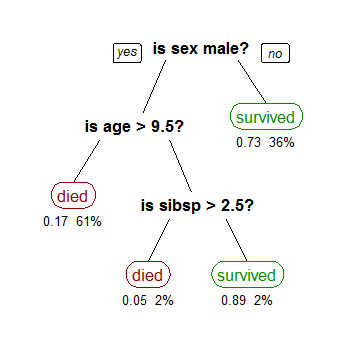
\includegraphics[height=.9\textheight]{../J-0x03/tree_titanic_survivors.png}}
    % https://commons.wikimedia.org/wiki/File:CART_tree_titanic_survivors.png
    % License: CC ASA 3.0 unported.

    \vspace{-28mm}\parbox{.4\textwidth}{\red{E.g., passengers died
        with probability .17 which is 61\% of observations}}

    %\vspace{-18mm}
    \prevwork{Stephen Milborrow}
\end{frame}

\begin{frame}{Quadtree}
  \cimgh{../J-0x03/500px-Point_quadtree.png}
\end{frame}

\begin{frame}{$kd$-tree}
  \cimgh{../J-0x03/370px-Kdtree_2d.png}  
\end{frame}

\begin{frame}{Random subspace methods}
  Draw $k$ hyperplanes at random.
  \begin{itemize}
  \item With text, dot product, so random planes through origin
  \item With nearly everything else, random planes period
  \end{itemize}

  Result: $\log(n)$ search time
\end{frame}

\begin{frame}
  \frametitle{Decision Trees}
  \only<1>{
    Variations
    \begin{itemize}
    \item Classification tree
    \item Regression tree
    \end{itemize}
    \bigskip
    CART = classification and regression trees
  }
  \only<2>{
    % https://www.pexels.com/photo/nature-bird-australia-owl-105810/
    % https://static.pexels.com/photos/105810/pexels-photo-105810.jpeg
    % CC0 license
    \vspace{-3cm}
    \cimgwb{../J-0x03/owl.jpg}
    \vspace{-8.7cm}
    \phrase{What can go wrong?}
  }
  \only<3>{
    Ensemble methods
    \begin{itemize}
    \item Bagging
    \item Random forest
    \item \gray{Boosted trees \textit{ (gradient boosted trees)}}
    \item \gray{Rotation forest}
    \end{itemize}
  }
\end{frame}

\begin{frame}{Boostrap aggregating = bagging}
  \only<1>{
    Bagging
    \begin{itemize}
    \item Increase stability
    \item Increase accuracy
    \item Reduce variance
    \item Avoid overfitting
    \end{itemize}
    A type of model averaging (ensemble method).
  }
  \only<2>{
    \begin{itemize}
    \item Training set $D$ of size $n$
    \item Sample $D$ \textit{with replacement} to create $D_1, \ldots, D_k$ of size $n'$
    \item If $n=n'$, expect $1-1/e \approx 63.2\%$ repeats
    \end{itemize}
    \begin{itemize}
    \item Train $k$ models
    \item Average (regression) or vote (classification)
    \end{itemize}
  }
\end{frame}

\begin{frame}
  \frametitle{Random subspace method}
  \only<1>{
    \phrase{attribute bagging = feature bagging}
  }
  \only<2>{
    \blue{Bagging (bootstrap aggregation)} = resampling to create more
    data sets, train models on different samples

    \blue{Attribute bagging} = project to create more data sets, train
    models on different samples
  }
\end{frame}

\begin{frame}
  \frametitle{Random forests}
  \only<1>{
    \vspace{1cm}
    \centerline{Combine \blue{bagging} with \blue{random subspace method}}
  }
\end{frame}

%%%%%%%%%%%%%%%%%%%%%%%%%%%%%%%%%%%%%%%%%%%%%%%%%%%%%%%%%%%%%%%%%%%%%%
%\talksection{Break}

\begin{frame}
  % https://www.pexels.com/photo/branches-fog-forest-landscape-235635/
  % https://static.pexels.com/photos/235635/pexels-photo-235635.jpeg
  % CC0 license
  \cimgwb{../J-0x03/forest.jpg}
  \vspace{-9cm}
  \phrase{questions?}
\end{frame}

%%%%%%%%%%%%%%%%%%%%%%%%%%%%%%%%%%%%%%%%%%%%%%%%%%%%%%%%%%%%%%%%%%%%%%
%\talksection{Break}

\talksection{Images}

\begin{frame}{Images}
  \only<1>{
    \phrase{Signal processing}

    \vspace{1cm}
    \centerline{in 2 or 3 dimensions}
  }
  \only<2>{
    Details that can matter:
    \begin{itemize}
    \item Illumination
    \item White balance
    \item Resolution
    \item Camera settings (e.g., depth of field)
    \item Sensor noise
    \item Compression technology
    \end{itemize}
  }
  \only<3>{
    Challenges:
    \begin{itemize}
    \item Segmentation
    \item Area of interest detection
    \item Perspective shifting
    \end{itemize}
  }
  \only<4>{
    Applications:
    \begin{itemize}
    \item Agriculture: fruit ripening, automated harvesting
    \item Security: detecting specific people
    \item Security: detecting accidents (e.g., falls)
    \item Art: counterfeit detection
    \item Medicine: assisted surgery
    \item Image search
    \end{itemize}
  }
  \only<5>{
    Image search (at first):
    \begin{itemize}
    \item Texture
    \item Colour
    \item Shape, simple objects
    \end{itemize}
  }
\end{frame}

\begin{frame}
  \cimg{brisk-image-descriptors.png}
  \prevwork{Eddie Bell @ Lyst}
\end{frame}

\begin{frame}
  \cimg{results-1.png}
  \prevwork{Eddie Bell @ Lyst}
\end{frame}

\begin{frame}
  \cimg{results-2.png}
  \prevwork{Eddie Bell @ Lyst}
\end{frame}

\begin{frame}
  \cimg{results-3.png}
  \prevwork{Eddie Bell @ Lyst}
\end{frame}

\begin{frame}
  \cimg{image-filter.png}
\end{frame}

\begin{frame}
  \cimgh{word2vec-1.png}
\end{frame}

\begin{frame}
  \cimghh{word2vec-2.png}
  \prevwork{Eddie Bell @ Lyst}
\end{frame}

\begin{frame}
  \cimg{brain-1.png}
  \prevwork{Google?}
\end{frame}

\begin{frame}
  \cimg{brain-2.png}
  \prevwork{Google?}
\end{frame}


%%%%%%%%%%%%%%%%%%%%%%%%%%%%%%%%%%%%%%%%%%%%%%%%%%%%%%%%%%%%%%%%%%%%%%
%\talksection{Break}

\begin{frame}
  % https://www.pexels.com/photo/grayscale-photo-of-chair-inside-the-establishment-162389/
  % https://static.pexels.com/photos/162389/lost-places-old-decay-ruin-162389.jpeg
  % CC0 license
  \cimgwb{chair.jpg}
  \vspace{-10.2cm}
  \phrase{\hspace{16mm}questions?}
\end{frame}


%%%%%%%%%%%%%%%%%%%%%%%%%%%%%%%%%%%%%%%%%%%%%%%%%%%%%%%%%%%%%%%%%%%%%%
%\talksection{Break}

\talksection{PCA}

\begin{frame}
  \phrase{Principle component analysis}

  \sphrase{Analyse en composantes principales}
\end{frame}

\begin{frame}
  \frametitle{Motivation}
  \phrase{Remember the Curse of Dimensionality?}
\end{frame}

\begin{frame}[t]
  \frametitle{Principle}

  \vspace{1cm}
  \begin{itemize}
  \item Linear transformations have axes
  \item Find them (eigenvectors of the covariance matrix)
  \item Pick the biggest ones
  \end{itemize}

  \vspace{5mm}
  \only<2>{\phrase{Fitting an $n$-dimensional ellipsoid to the data}}
\end{frame}

\begin{frame}
  \frametitle{Uses}
  \begin{itemize}
  \item Exploratory data analysis
  \item Compression
  \end{itemize}
\end{frame}

\begin{frame}
  \frametitle{Also known as}
  \begin{itemize}
  \item Discrete Kosambi-Karhunen–Loève transform (KLT) (signal processing)
  \item Hotelling transform (multivariate quality control)
  \item Proper orthogonal decomposition (POD) (ME)
  \item Singular value decomposition (SVD), Eigenvalue decomposition (EVD) (linear algebra)
  \item Etc.
  \end{itemize}
\end{frame}

\begin{frame}
  \frametitle{History}
  \begin{itemize}
  \item Invented by Karl Pearson in 1901
  \item Invented (again) and named by Harold Hotelling in 1930's
  \item Also known as\dots
  \end{itemize}
\end{frame}

\begin{frame}
  \frametitle{Also known as}

  \begin{itemize}
  \item It's a long list, every field uses a different name\dots
  \end{itemize}
\end{frame}

\begin{frame}{In addition to PCA\dots}
  There are newer methods that are sometimes better.

  \begin{itemize}
  \item Sometimes they are faster.
  \item Sometimes the projection makes more sense.
  \end{itemize}

  $t$-SNE is the most common you'll encounter.
\end{frame}

%%%%%%%%%%%%%%%%%%%%%%%%%%%%%%%%%%%%%%%%%%%%%%%%%%%%%%%%%%%%%%%%%%%%%%
%\talksection{Break}

\begin{frame}
  % https://www.pexels.com/photo/macro-shot-of-purple-flower-144282/
  % https://static.pexels.com/photos/144282/pexels-photo-144282.jpeg
  % CC0 license
  \cimgwb{blue-flowers.jpg}
  \vspace{-9cm}
  \wphrase{questions?}
\end{frame}


%%%%%%%%%%%%%%%%%%%%%%%%%%%%%%%%%%%%%%%%%%%%%%%%%%%%%%%%%%%%%%%%%%%%%%
%\talksection{Break}


\end{document}
